% author:   sam tenka
% change:   2022-05-11
% create:   2022-05-11

%==============================================================================
%=====  0.  DOCUMENT SETTINGS  ================================================
%==============================================================================

%~~~~~~~~~~~~~~~~~~~~~~~~~~~~~~~~~~~~~~~~~~~~~~~~~~~~~~~~~~~~~~~~~~~~~~~~~~~~~~
%~~~~~~~~~~~~~  0.0. About and Beyond this Exposition  ~~~~~~~~~~~~~~~~~~~~~~~~

%---------------------  0.0.0. page geometry  ---------------------------------
\documentclass[11pt, justified]{tufte-book}
\geometry{
  left           = 0.90in, % left margin
  textwidth      = 4.95in, % main text block
  marginparsep   = 0.15in, % gutter between main text block and margin notes
  marginparwidth = 2.30in, % width of margin notes
                 % 0.20in  % width from margin to edge
}

%---------------------  0.0.1. math packages  ---------------------------------
\newcommand\hmmax{0}
\newcommand\bmmax{0}
\usepackage{amsmath, amssymb, amsthm, mathtools, bm, euler}
\usepackage{listings}

%---------------------  0.0.2. graphics packages  -----------------------------
\usepackage{graphicx, xcolor}
\usepackage{enumitem}\setlist{nosep}
\usepackage{float, capt-of}

%~~~~~~~~~~~~~~~~~~~~~~~~~~~~~~~~~~~~~~~~~~~~~~~~~~~~~~~~~~~~~~~~~~~~~~~~~~~~~~
%~~~~~~~~~~~~~  0.1. Header Formatting  ~~~~~~~~~~~~~~~~~~~~~~~~~~~~~~~~~~~~~~~

\definecolor{mgrn}{rgb}{0.15, 0.65, 0.05} \newcommand{\grn}{\color{mgrn}}
\definecolor{mred}{rgb}{0.90, 0.05, 0.05} \newcommand{\red}{\color{mred}}
\definecolor{mblu}{rgb}{0.05, 0.35, 0.70} \newcommand{\blu}{\color{mblu}}
\definecolor{mbre}{rgb}{0.30, 0.45, 0.60} \newcommand{\bre}{\color{mbre}}
\definecolor{mgre}{rgb}{0.55, 0.55, 0.50} \newcommand{\gre}{\color{mgre}}

%\newcommand{\note}[1]{{\blu \textsf{#1}}}
\newcommand{\attn}[1]{{\red \textsf{#1}}}

%---------------------  0.1.0. tidbit headers  --------------------------------
\newcommand{\samtitle} [1]{
  \par\noindent{\Huge \sf \blu #1}
  \vspace{0.4cm}
}

\newcommand{\samquote} [2]{
    \marginnote[-0.4cm]{\begin{flushright}
    \scriptsize
        \gre {\it #1} \\ --- #2
    \end{flushright}}
}

%---------------------  0.1.1. section headers  -------------------------------

\newcommand{\samsection} [1]{
  \vspace{0.5cm}
  \par\noindent{\LARGE \sf \blu #1}
  \vspace{0.1cm}\par
}

\newcommand{\samsubsection}[1]{
  \vspace{0.3cm}
  \par\noindent{\large \sf \bre #1}
  \vspace{0.1cm}\par
}

\newcommand{\samsubsubsection}[1]{
   \vspace{0.1cm}
   \par\noindent{\hspace{-2cm}\normalsize \sc \gre #1} ---
}

%---------------------  0.1.2. clear the bibliography's header  ---------------
\usepackage{etoolbox}
\patchcmd{\thebibliography}{\section*{\refname}}{}{}{}

%~~~~~~~~~~~~~~~~~~~~~~~~~~~~~~~~~~~~~~~~~~~~~~~~~~~~~~~~~~~~~~~~~~~~~~~~~~~~~~
%~~~~~~~~~~~~~  0.2. Math Symbols and Blocks  ~~~~~~~~~~~~~~~~~~~~~~~~~~~~~~~~~

%---------------------  0.2.0. probability symbols  ---------------------------
\newcommand{\KL}{\text{KL}}
\newcommand{\EN}{\text{H}}
\newcommand{\note}[1]{{\blu \textsf{#1}}}

\newcommand{\scirc}{\mathrel{\mathsmaller{\mathsmaller{\mathsmaller{\circ}}}}}
\newcommand{\cmop}[2]{{(#1\!\to\!#2)}}

% losses averaged in various ways: 
\newcommand{\Ein}  {\text{trn}_{\Ss}}
\newcommand{\Einb} {\text{trn}_{\check\Ss}}
\newcommand{\Einc} {\text{trn}_{\Ss\sqcup \check\Ss}}
\newcommand{\Egap} {\text{gap}_{\Ss}}
\newcommand{\Eout} {\text{tst}}



%---------------------  0.2.1. double-struck and caligraphic letters  ---------
\newcommand{\Aa}{\mathbb{A}}\newcommand{\aA}{\mathcal{A}}
\newcommand{\Bb}{\mathbb{B}}\newcommand{\bB}{\mathcal{B}}
\newcommand{\Cc}{\mathbb{C}}\newcommand{\cC}{\mathcal{C}}
\newcommand{\Dd}{\mathbb{D}}\newcommand{\dD}{\mathcal{D}}
\newcommand{\Ee}{\mathbb{E}}\newcommand{\eE}{\mathcal{E}}
\newcommand{\Ff}{\mathbb{F}}\newcommand{\fF}{\mathcal{F}}
\newcommand{\Gg}{\mathbb{G}}\newcommand{\gG}{\mathcal{G}}
\newcommand{\Hh}{\mathbb{H}}\newcommand{\hH}{\mathcal{H}}
\newcommand{\Ii}{\mathbb{I}}\newcommand{\iI}{\mathcal{I}}
\newcommand{\Jj}{\mathbb{J}}\newcommand{\jJ}{\mathcal{J}}
\newcommand{\Kk}{\mathbb{K}}\newcommand{\kK}{\mathcal{K}}
\newcommand{\Ll}{\mathbb{L}}\newcommand{\lL}{\mathcal{L}}
\newcommand{\Mm}{\mathbb{M}}\newcommand{\mM}{\mathcal{M}}
\newcommand{\Nn}{\mathbb{N}}\newcommand{\nN}{\mathcal{N}}
\newcommand{\Oo}{\mathbb{O}}\newcommand{\oO}{\mathcal{O}}
\newcommand{\Pp}{\mathbb{P}}\newcommand{\pP}{\mathcal{P}}
\newcommand{\Qq}{\mathbb{Q}}\newcommand{\qQ}{\mathcal{Q}}
\newcommand{\Rr}{\mathbb{R}}\newcommand{\rR}{\mathcal{R}}
\newcommand{\Ss}{\mathbb{S}}\newcommand{\sS}{\mathcal{S}}
\newcommand{\Tt}{\mathbb{T}}\newcommand{\tT}{\mathcal{T}}
\newcommand{\Uu}{\mathbb{U}}\newcommand{\uU}{\mathcal{U}}
\newcommand{\Vv}{\mathbb{V}}\newcommand{\vV}{\mathcal{V}}
\newcommand{\Ww}{\mathbb{W}}\newcommand{\wW}{\mathcal{W}}
\newcommand{\Xx}{\mathbb{X}}\newcommand{\xX}{\mathcal{X}}
\newcommand{\Yy}{\mathbb{Y}}\newcommand{\yY}{\mathcal{Y}}
\newcommand{\Zz}{\mathbb{Z}}\newcommand{\zZ}{\mathcal{Z}}

\newcommand{\sfa}{\mathsf{a}}\newcommand{\fra}{\mathcal{a}}
\newcommand{\sfb}{\mathsf{b}}\newcommand{\frb}{\mathcal{b}}
\newcommand{\sfc}{\mathsf{c}}\newcommand{\frc}{\mathcal{c}}
\newcommand{\sfd}{\mathsf{d}}\newcommand{\frd}{\mathcal{d}}
\newcommand{\sfe}{\mathsf{e}}\newcommand{\fre}{\mathcal{e}}
\newcommand{\sff}{\mathsf{f}}\newcommand{\frf}{\mathcal{f}}
\newcommand{\sfg}{\mathsf{g}}\newcommand{\frg}{\mathcal{g}}
\newcommand{\sfh}{\mathsf{h}}\newcommand{\frh}{\mathcal{h}}
\newcommand{\sfi}{\mathsf{i}}\newcommand{\fri}{\mathcal{i}}
\newcommand{\sfj}{\mathsf{j}}\newcommand{\frj}{\mathcal{j}}
\newcommand{\sfk}{\mathsf{k}}\newcommand{\frk}{\mathcal{k}}
\newcommand{\sfl}{\mathsf{l}}\newcommand{\frl}{\mathcal{l}}
\newcommand{\sfm}{\mathsf{m}}\newcommand{\frm}{\mathcal{m}}
\newcommand{\sfn}{\mathsf{n}}\newcommand{\frn}{\mathcal{n}}
\newcommand{\sfo}{\mathsf{o}}\newcommand{\fro}{\mathcal{o}}
\newcommand{\sfp}{\mathsf{p}}\newcommand{\frp}{\mathcal{p}}
\newcommand{\sfq}{\mathsf{q}}\newcommand{\frq}{\mathcal{q}}
\newcommand{\sfr}{\mathsf{r}}\newcommand{\frr}{\mathcal{r}}
\newcommand{\sfs}{\mathsf{s}}\newcommand{\frs}{\mathcal{s}}
\newcommand{\sft}{\mathsf{t}}\newcommand{\frt}{\mathcal{t}}
\newcommand{\sfu}{\mathsf{u}}\newcommand{\fru}{\mathcal{u}}
\newcommand{\sfv}{\mathsf{v}}\newcommand{\frv}{\mathcal{v}}
\newcommand{\sfw}{\mathsf{w}}\newcommand{\frw}{\mathcal{w}}
\newcommand{\sfx}{\mathsf{x}}\newcommand{\frx}{\mathcal{x}}
\newcommand{\sfy}{\mathsf{y}}\newcommand{\fry}{\mathcal{y}}
\newcommand{\sfz}{\mathsf{z}}\newcommand{\frz}{\mathcal{z}}


      \newcommand{\phdot}{\phantom{.}}

%---------------------  0.2.2. math environments  -----------------------------
\newtheorem*{qst}{Question}
\newtheorem*{thm}{Theorem}
\newtheorem*{lem}{Lemma}
% ...
\theoremstyle{definition}
\newtheorem*{dfn}{Definition}

%~~~~~~~~~~~~~~~~~~~~~~~~~~~~~~~~~~~~~~~~~~~~~~~~~~~~~~~~~~~~~~~~~~~~~~~~~~~~~~
%~~~~~~~~~~~~~  0.3. Section Headers  ~~~~~~~~~~~~~~~~~~~~~~~~~~~~~~~~~~~~~~~~~


\begin{document}
\samtitle{mlentary (6.86x)}

  \marginnote[-0.05cm]{%
    \textsc{Table of Contents}
    \begin{description}
      %\item[] \vphantom{.} 
      %  \begin{description}
      %  \end{description}
      \item[prologue] \phdot 
        \begin{description}
          \item[bird's eye framework] \phdot
          \item[flooding plains] \phdot
          \item[pairing flavors] \phdot
          \item[ancient tablets] \phdot
        \end{description}
      \item[linear classification] \phdot
        \begin{description}
          \item[linear approximations] \phdot % hypothesis class; briefly mention regression
          \item[iterative optimization] \phdot % perceptron, logistic
          \item[generalization bounds] \phdot % generalization bounds
          \item[model selection] \phdot % validation, featurization from domain knowledge, which objective func?
          \item[priors and generalization] \phdot % priors and regularization
          \item[continuous optimization] \phdot % convex optimization; implicit regularization
          \item[kernels enrich approximations] \phdot
        \end{description}
      \item[nonlinearities] \phdot
        \begin{description}
          \item[fixed featurization] \phdot % classic nonlinearities: discrete-continuous (softmax; embedding); normalization; binning 
          \item[learned featurizations] \phdot
          \item[differentiation] \phdot % smoothness assumption, backprop as dynaprog, autodiff
          \item[architecture and symmetry] \phdot % CNNs, RNNs
          \item[feature hierarchies] \phdot % 
          \item[stochastic gradient descent] \phdot % learning rates as riemannian metrics; conditioning; annealing
          \item[loss landscape shape] \phdot % thinking about minima etc
        \end{description}
      \item[structured inference] \phdot
        \begin{description}
          \item[graphical generative models] \phdot % directed models
          \item[inferring conditional marginals] \phdot
          \item[learning parameters] \phdot % spectre of marginal likelihood; EM, other variational methods, MCMC
          \item[hierarchy and mixtures] \phdot
          \item[hierarchy and transfer] \phdot
          \item[variational and sampling methods] \phdot % - tie in with deep learning 
          \item[amortized inference] \phdot % - tie in with deep learning 
        \end{description}
      \item[reductions to supervision] \phdot
        \begin{description}
          \item[to build a tool, use it] \phdot
          \item[distributions as maps] \phdot
          \item[self-supervised: ] \phdot
          \item[self-supervised: ] \phdot
          \item[reinforcement: ] \phdot
          \item[reinforcement: ] \phdot
              % another paradigm: learning-from-instruction
          \item[beyond i.i.d.] \phdot
        \end{description}
      \item[appendices] \phdot 
        \begin{description}
          \item[python refresher] \phdot
          \item[math refresher] \phdot
          \item[notes on high dimensions] \phdot
          \item[notes on bayes' law] \phdot
        \end{description}
    \end{description}
  }
   
  \samsection{a prologue} %in three examples}

    \samsubsection{bird's eye framework}% data flow and goals 
    What tools can we use to automatically extract, extrapolate, and explain
    patterns in data?

    \newpage
    Now comes a hurried tour of the sorts of analysis we'll do.  \attn{Please
    skim} the remainder of this prologue without trying to understand each
    step.

    \samsubsection{flooding plains}

    \begin{marginfigure}
        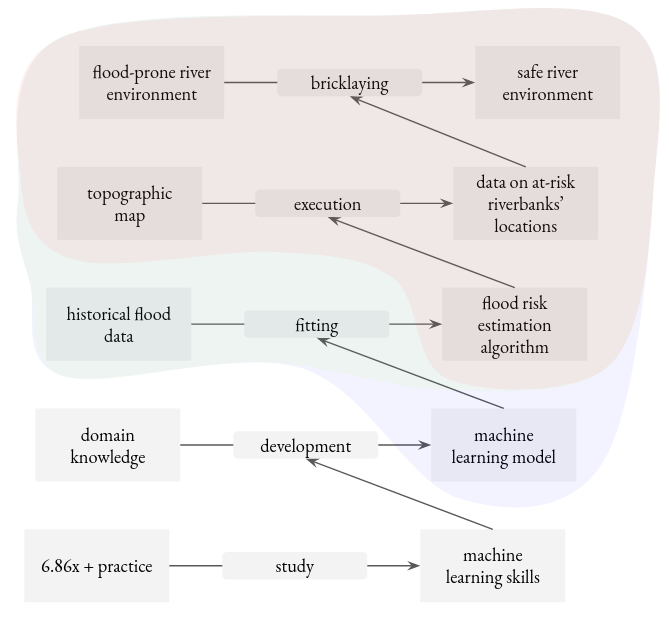
\includegraphics[width=1.0\textwidth]{seven-days}
        \caption{%
          Machine learning continues our human tradition toward the systematic and automatic.
          %
          What for one generation is a luckily discovered idea or recipe
          (bottom tip of red), the next generation refines by
          careful human thought (green). 
          %
          What to one generation is a task (green) requiring human thought
          is to a future generation merely a routine parameterized by some
          newly discovered recipe (bottom tip of blue).
          %
          And the cycle repeats.
          %
          %%\textbf{Left} column: assumed given.
          %%\textbf{Middle} column: activities in the past done by humans and in the future done by machine.
          %%\textbf{Right} column: artifacts valuable either directly (top right corner) or because they help (via diagonal arrows) achieve more direct goals. 
        }
    \end{marginfigure}

    \samsubsubsection{a whimsical story about automation}
      We automate when we re-cast the previous generation's \emph{methods} as
      mere \emph{data} to generate and manipulate. 

      We once sought safety from floods.  Long ago, if we lived near safe
      riverbanks it was by luck; we then found we could make unsafe rivers safe
      by erecting floodwalls.  This was dangerous work, so we built brick
      laying robots to do the hard part.  The machines needed as input some
      flood-risk estimates: the location and mud-softnesses of the river banks to
      work on.

      So we sought flood-risk estimates.  At first, if our city's flood-risk
      estimates were correct it was by luck; we then found we could translate
      topographic maps to flood-risk estimates by applying geology ideas.  This
      was tedious work, so we built computers to do the hard part.  The
      computers needed as input a risk-estimation \emph{algorithm}: a recipe of
      the geology rules to calculate through.

      We thus sought risk-estimation algorithms.  At first, if our research
      center's risk-estimation algorithms were robust to new landscapes it was
      by luck; we then found we could calibrate our algorithms to historical
      flood data from many cities.  To find the better of two candidate
      algorithms, we had to aggregate all their many small success and errors.
      This was subtle work, so we developed statistical theories to do the hard
      part.  The theories needed as input a machine learning model: a class of
      candidates.

      We thus sought machine learning models.  At first, if our machine
      learning models were highly predictive it was by luck; we then found
      general principles to guide model design and selection from domain
      knowledge.

      It is these principles that we study in 6.86x.

      Looking back, these are principles that produce machine learning models
      that produce risk-estimation algorithms that produce flood-risk estimates
      that guide the building of floodwalls. 

    %%values have expanded from
    %%\emph{lucky} such as the dryness of not being flooded, to 
    %%\emph{chores} such as installing floodwalls along a river, to
    %%\emph{data} that informs those chores, such as where along the river floods the worst, and on to 
    %%\emph{algorithms} that transform data (say, a topographical map) to more useful forms (say, flood risk zones).
    %%People working in insurance and law and have for centuries written such algorithms by hand.
    %%\emph{algorithms that output algorithms}.
    %%%
    %%In the beginning, we had concrete \emph{chores} such as the milling of
    %%wheat.
    %%%
    %%Then there was \emph{data}, which helped a person to accomplish chores by 
    %%teaching them methods and alerting them to relevant aspects of the environment.
    %%Discovering and recording such data was so useful that some folk did that as
    %%their full time job.
    %%%
    %%Then we invented computer \emph{programs} to transform data to more useful
    %%forms.  
    %%%
    %%Then came \emph{programs} that write programs.  
    %%%
    %%What will we continue on to create?

  \samsection{linear models}
    \samsubsection{linear approximations} 
    \samsubsection{iterative optimization} 
    \samsubsection{generalization bounds} 
    \samsubsection{model selection} 
    \samsubsection{priors and generalization} 
    \samsubsection{continuous optimization} 
    \samsubsection{kernels enrich approximations} 


  \samsection{nonlinearities}
    \samsubsection{fixed featurization} 
    \samsubsection{learned featurizations} 
    \samsubsection{differentiation} 
    \samsubsection{architecture and symmetry} 
    \samsubsection{feature hierarchies} 
    \samsubsection{stochastic gradient descent} 
    \samsubsection{loss landscape shape} 


  \samsection{structured inference}
    \samsubsection{graphical generative models} 
    \samsubsection{inferring conditional marginals} 
    \samsubsection{learning parameters} 
    \samsubsection{hierarchy and mixtures} 
    \samsubsection{hierarchy and transfer} 
    \samsubsection{variational and sampling methods} 
    \samsubsection{amortized inference} 

  \samsection{reductions to supervision}
    \samsubsection{beyond the i.i.d.\ hypothesis}
    \samsubsection{to build a tool, use it} 
    \samsubsection{distributions as maps} 
    \samsubsection{self-supervised: } 
    \samsubsection{self-supervised: } 
    \samsubsection{reinforcement: } 
    \samsubsection{reinforcement: } 

      \samsubsubsection{out-of-distribution tests}
      \samsubsubsection{dependent samples}
      \samsubsubsection{causality}

  \samsection{appendices}
    Here are ``refreshers'' on programming and on math, especially on the
    math of high dimensions and of bayes' law.
    They can help jog your memory of the math and
    programming preparation you should have done in preparation for
    6.86x.\marginnote{%
      Depending on your background and personality, you might recognize and
      care that throughout these notes we are a bit sloppy with our probability
      and programming.  No standard compiler can compile our pseudocode;
      likewise, our theorems are actually theorem sketches in need of
      additional analytic hypotheses. 
      %
      For readers so concerned, we assume an additional prerequisite: enough
      technical background that we may leave implicit both the articulation of
      measure-theory technicalities and the implementation of pseudocode.
    }
    They also help establish our naming conventions.  The refreshers are meant
    neither to explain these topics nor to provide a complete outline of
    prerequisites.

    \samsubsection{python programming refresher}
      \samquote{
          \begin{flushleft}
          \texttt{\phantom{}def get\_random\_number():} \\
          \texttt{\phantom{....}return 4 \# chosen by a fair dice roll} \\
          \texttt{\phantom{.............}\# guaranteed to be random}
          \end{flushleft}\phantom{.}
      }{xkcd, Randall Munroe, translated to Python}

      \samsubsubsection{setup}
      \samsubsubsection{state and control flow}
      \samsubsubsection{input/output}
      \samsubsubsection{numpy}

    \samsubsection{math notation and refresher}
      \samquote{
        He had bought a large map representing the sea, \\
        Without the least vestige of land: \\
        And the crew were much pleased when they found it to be \\
        A map they could all understand.
      }{The Hunting of the Snark, Charles Dodgson}

      \samsubsubsection{probability}
        We've tried to use 
          \vspace{-0.10cm}
        $$
          \text{\textsf{sans serif} for the names of random variables,}
          \vspace{-0.15cm}
        $$
        $$
          \text{\emph{italics} for the values they may take, and}
        $$
        $$
          \text{$\mathcal{CURLY~CAPS}$ for sets of such values.} 
        $$
        For example, we write $p_{\sfy|\sfh}(y|h)$ for the probability that the
        random variable $\sfy$ takes the value $y$ conditioned on the event that
        the random variable $\sfh$ takes the value $h$.
        %
        Likewise, our notation $p_{\hat \sfh|\sfh}(h|h)$ indicates the
        probability that the random variables $\hat \sfh$ and $\sfh$ agree in
        value given that $\sfh$ takes a value $h\in \hH$.
      \samsubsubsection{linear algebra}

      \samsubsubsection{calculus}
      \samsubsubsection{higher dimensions}

    \samsubsection{high dimensional geometry}
      \samquote{
        Can I just say Chris for one moment that I have a new theory about the
        brontosaurus. ...  This theory goes as follows and begins now. All
        brontosauruses are thin at one end, much, much thicker in the middle
        and then thin again at the far end. That is my theory, it is mine, and
        belongs to me and I own it, and what it is too.
      }{Flying Circus, Monty Python}

      \samsubsubsection{concentration of measure}

        \begin{lem}[Chernoff]
            The fraction of heads among $N$ i.i.d.\ flips of a biased coin
            exceeds its mean $p$ by $g$ with chance at most 
            $\exp(-Ng^2)$, for $0 \leq p < p+g \leq 1$.
        \end{lem}
        \vspace{-0.5cm}
        \begin{figure}[h]
            \centering
            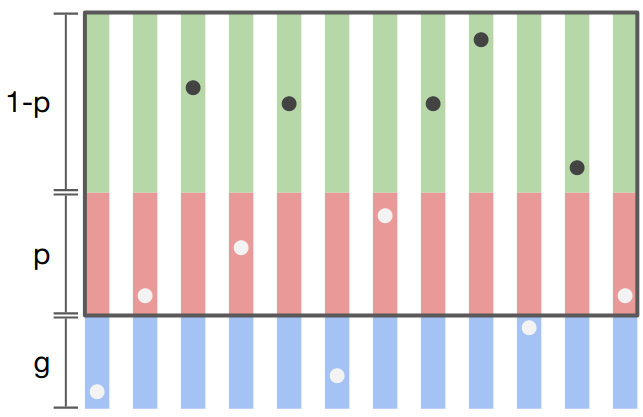
\includegraphics[height=4cm, clip]{chernoff}
            \caption{{
                We sample points uniformly at random on $N$
                sticks, each with three parts: \textbf{green}
                with length $1-p$, \textbf{red} with length $p$, and
                \textbf{blue} with length $g$.  We call non-blue points
                \textbf{boxed} and non-green points \textbf{hollow}.
            }}
            \label{fig:chernoff}
        \end{figure}
        \vspace{-0.5cm}
        \begin{proof} \renewcommand{\qedsymbol}{}
            Let our coin flips arise from sampling points on sticks
            (Figure \ref{fig:chernoff}), where green means tails, red
            means heads, and we condition on the event that blues do not occur.
            %
            To show that less than $(p+g)N = p^\prime N$ flips are
            heads is to show --- given that all points are \textbf{boxed} ---
            that less than $p^\prime N$ points are red. 
            %
            For any $M$:
            {%
            \begin{align*}
                    & ~ \Pp[\text{$M$ are red $\mid$ all are boxed}] \\
                  = & ~ \frac{\Pp[\text{all hollows are red $\mid$ $M$ hollow}] \cdot \Pp[\text{$M$ are hollow}]}{\Pp[\text{all are boxed}] } \\
                  = & ~ (1 - g/p^\prime)^{M} \cdot (1+g)^{N} \cdot \Pp[\text{$M$ are hollow}]
            \end{align*}
            }%
            We sum over $M\geq p^\prime N$, bound $\Pp[\cdots p^\prime N \cdots] \leq 1$,
            then invoke $(x \mapsto x^{p^\prime})$'s concavity and
            $\exp$'s convexity:
            \begin{align*}
                &~\Pp[\text{at least $p^\prime N$ are red $\mid$ all are boxed}]
                \\ \leq
                &~(1 - g/p^\prime)^{p^\prime N} \cdot (1+g)^{N} \cdot \Pp[\text{at least $p^\prime N$ are hollow}]
                \\ \leq
                &~(1 - g)^N \cdot (1 + g)^{N}
                =
                (1 - g^2)^N
                \leq
                \exp(- Ng^2)
                ~~~~~\square
            \end{align*}
        \end{proof}
        \vspace{-0.5cm}
        The Chernoff bound gives us the control over tails we would expect from the
        Central Limit Theorem, but for finite instead of asymptotically large
        $N$.  In particular, when we learn from much but finite data, the
        training error will \textbf{concentrate} near the testing error.

        Indeed, for any $f\in \Hh$, $\Ein(f)$ is the average of $N$ independent 
        Bernoullis of mean $\Eout(f)$.  So for finite $\Hh$, the gap is
        probably small:
        \begin{align*}
            &~\Pp_{\Ss\sim \Dd^N}[\Egap(\Ll) \geq g] \\
            \leq 
            &~\sum_{f\in \Hh} \Pp_{\Ss\sim \Dd^N}[\Eout(f) \geq \Ein(f) + g] \\
            \leq
            &~|\Hh| \cdot \exp(-Ng^2)
        \end{align*}

        For example, if $\Hh$ is parameterized by $P$ numbers, each represented
        on a computer by $32$ bits, then $|\Hh|\leq 2^{32 P}$ and, with
        probability $1-\delta$, the gap is less than
        $$
            \sqrt{(\log(1/\delta) + 32 P)/N}
        $$
        This bound's sensitivity to the description length $32 P$ may seem
        artificial.  Indeed, the various $\Hh$ used in practice --- e.g.
        linear models or neural networks --- depend smoothly on their
        parameters, so the parameters' least significant bits barely affect 
        the classifier.  In other words, $\Hh$'s cardinality is not an apt
        measure of its size.  The VC-dimension measures $\Hh$ more subtly.


      \samsubsubsection{quadratic forms}
      \samsubsubsection{covariance, correlation, least squares regression}

    \samsubsection{bayesian inference}
      \samquote{So little of what could happen does happen.}{salvador dali}

      \samsubsubsection{conceptual framework}
      We're confronted with an observation or dataset $\sfo$ that comes from
      some unknown underlying pattern $\sfh$.  We know how each possible value
      $h$ for $\sfh$ induces a distribution on $\sfo$ and we have a prior sense
      of which $h$s are probable.  Bayes' law helps us update this sense to
      account for the dataset by relating two functions of $h$:
      $$
        \underbrace{p_{\sfh|\sfo}(h|o)}_{\text{posterior}}
        \propto
        \underbrace{p_{\sfo|\sfh}(o|h)}_{\text{likelihood}}
        \cdot
        \underbrace{p_{\sfh}(h)}_{\text{prior}}
      $$

      Bayes' law underlies most of our analyses throughout these
      notes.\marginnote{%
        Like Newton's $F=ma$, Bayes is by itself inert: to make predictions
        we'd have to specify our situation's forces or likelihoods.  Continuing
        the metaphor, we will rarely solve our equations exactly; we'll instead
        make approximations good enough to build bridges and swingsets.  Still,
        no one denies that $F=ma$ orients us usefully in the world of physics.
        So it is with the law of Bayes.
      }

      Formally, we posit a set $\hH$ of \emph{hypotheses}, a set $\oO$ of
      possible \emph{observations}, and a set $\aA$ of permitted
      \emph{actions}.  We assume as given a joint probability measure
      $p_{\sfo,\sfh}$ on $\oO\times \hH$ and a \emph{cost function}
      $c:\aA\times \hH \to \Rr$.
      %
      That cost function says how much it hurts to take the action $a\in \aA$
      when the truth is $h\in \hH$.
      %
      Our primary aim is to construct a map $\pi:\oO\to \aA$ that makes the
      expected cost $\Ee_{\sfh,\sfo} \, c(\pi(\sfa); \sfh)$ small.

      Below are three examples.  In each case, we're designing a robotic vacuum
      cleaner: $\hH$ contains possible floor plans; $\oO$, 
      possible readings from the robot's sensors.  The examples differ in how
      they define and interpret $\aA$ and $c$.

      \textbf{A}.  $\aA$ consists of probability distributions over $\hH$. We
      regard $\pi(o)$ as giving a posterior distribution on $\hH$ upon
      observation $o$.  Our cost $c(a;h)$ measures the surprise of someone who
      believes $a$ upon learning that $h$ is true. 
      %
      Such \emph{inference problems}, being in a precise sense universal, pose
      huge computational difficulties; we thus often collapse distributions to
      points, giving rise to the distinctive challenge of balancing estimation
      error with structural error.

      \textbf{B}.
      $\aA$ consists of latitude-longitude pairs, interpreted as a guessed
      location of the robot's charging station.  The cost $c(a;h)$ measures how
      distant our guess is from the truth.  
      %
      Such \emph{estimation problems} abound in science and engineering; they
      pose the distinctive challenge of balancing
      sensitivity-to-misleading-outliers against
      sensitivity-to-informative-datapoints.
      %robustness to measurement noise with
      %centeredness. 

      \textbf{C}.  $\aA$ consists of instructions we may send to the motors,
      instructions that induce motion through our partially-known room.  The
      cost $c(a;h)$ incentivizes motion into dusty spaces and penalizes bumping
      into walls.
      %
      We often compose such \emph{decision problems} sequentially; this gives
      rise to the distinctive challenge of balancing exploration with
      exploitation.

      \samsubsubsection{effect of prior choice}
      \samsubsubsection{mixture priors and hierarchy}

      \samsubsubsection{frequentism and choice of prior}
      %\samquote{
      %  I am wiser [than he] ... for
      %  ... he fancies he knows something 
      %  ... whereas I ... do not fancy I do.
      %}{socrates}
      %\samsubsubsection{uniform priors} % jeffries
        Our engineering culture prizes not just \emph{utility} but also
        \emph{confidence}, since strong guarantees on our designs allow 
        composition of our work into larger systems: equality, unlike
        similarity, is transitive.  For example, we'd often prefer a 99\%
        guarantee of adequate performance over a 90\% guarantee of ideal
        performance.  This asymmetry explains our pessimistic obsession with
        worst-case bounds over best-case bounds, cost functions over fitness
        functions, and simple models with moderate-but-estimatable errors over
        rich models with unknownable-but-often-small errors.

        The \emph{frequentist} or \emph{distribution-free} style of statistics
        continues this risk-averse tradition.  In the fullest instance of this
        style, we do inference as if the true unknown prior on $\hH$ is chosen
        adversarially.
        %
        That is, we try to find $\pi$ that makes the following error small:
        $$
          \max_{p_{\sfh}}
          \,
          \Ee_{\sfh \sim p_{\sfh}(\cdot)} \Ee_{\sfo \sim p_{\sfo}(\cdot|\sfh)}
          \,
          c(\pi(\sfo); \sfh) 
        $$
        %
        %For example, suppose $\aA=\hH$ and $c(a;h) = [\![a\neq h]\!]$ is the
        %zero-one cost.
        %The prior in the minimax pair $(\pi, p_{\sfh})$ tends to be pretty
        %uniform. 
        Intuitively, 

        %minimax 
        %``uniform'' prior
        %on hypothesis space.

      \samsubsubsection{p-hacking} % likelihoods, confidence intervals 
      \samsubsubsection{hidden assumptions} % distribution-existence as coherence condition

      \samsubsubsection{(multiple) hypothesis testing}
      %\samquote{
      %  The theory of probabilities is at bottom nothing but common sense
      %  reduced to calculus; it enables us to appreciate with exactness
      %  [what we] feel with a sort of instinct ...
      %}{pierre simon laplace}

      Let's now consider the case where $\hH$ is a small and finite.  We

      


\end{document}
%
%      \item[Statistics] .
%        \begin{description}
%          \item[bayesian inference] .
%          \item[hypothesis testing] .
%          \item[covariance] .
%          \item[gradient descent] .
%        \end{description}
%      \item[High Dimensions] .
%        \begin{description}
%          \item[geometry] .
%          \item[clusters and classes] .
%          \item[graphical models] .
%          \item[boosted trees] .
%        \end{description}
          %\item[contaminated faucets] .
          %\item[contaminated faucets] .

